\documentclass[9pt, a4paper]{article}

\usepackage{graphicx}
\usepackage{listings}
\usepackage{color}
\usepackage{amsmath}
\usepackage{geometry}
\usepackage{setspace}
\usepackage{biblatex}
\usepackage{float}
\usepackage[hidelinks]{hyperref}
\usepackage{subcaption}
\usepackage[export]{adjustbox}
\usepackage[normalem]{ulem}
\usepackage{wrapfig}
\usepackage{gensymb}

\addbibresource{citations.bib}
 
% Page master configuration
\lstset { basicstyle=\ttfamily, breaklines = true, tabsize=2 }
\geometry { a4paper, total={170mm,257mm}, left=20mm, top=20mm, right=20mm, bottom=20mm }
\graphicspath{{Images/}}
\addbibresource{biblography.bib}
\setlength{\parskip}{0.5em}
\setlength{\parindent}{0cm}
\setlength{\belowcaptionskip}{-10pt}

\definecolor{dkgreen}{rgb}{0,0.6,0}
\definecolor{gray}{rgb}{0.5,0.5,0.5}
\definecolor{mauve}{rgb}{0.58,0,0.82}

\lstset{frame=tb,
  language=Java,
  aboveskip=3mm,
  belowskip=3mm,
  showstringspaces=false,
  columns=flexible,
  basicstyle={\footnotesize\ttfamily},
  numbers=none,
  numberstyle=\tiny\color{gray},
  keywordstyle=\color{blue},
  commentstyle=\color{dkgreen},
  stringstyle=\color{mauve},
  breaklines=true,
  breakatwhitespace=true,
  tabsize=3
}

%%%%%%%%%%%%%%%%%%%%%%%%%%%%%%%%%%%%%%%%%%%%%%%%%%%%%%%%%%%%%%%%%%%%%%%%%%%%%%%%%%%%%%%%%%%%%%%%%%%%%%%%%%
\begin{document}

\begin{titlepage}
	\newcommand{\HRule}{\rule{\linewidth}{0.5mm}}
    
\includegraphics[scale=0.1]{./Images/Imperial_Logo.jpg} 
    \\
    \center 
	\textsc{\large Department of Electrical and Electronic Engineering }\\[0.5cm] 
	\textsc{\normalsize ELEC60030: Robotic Manipulation}\\[0.5cm] 
    
	\HRule \\[0.4cm]
	Team Machina: OpenMANIPULATOR-X Coursework Report
    \HRule \\[1.5cm]
     
    \begin{center}
		\underline{Authors}\\[0.5cm] 
        Khayle Torres \\ CID: 01753211 \\ kt1719@ic.ac.uk \\ [0.5cm]

        Xin Wang \\ CID: 01735253 \\ xw2519@ic.ac.uk \\ [0.5cm]
        
        Yuna Valade \\ CID: 01765409 \\ yv19@ic.ac.uk \\ [0.5cm]

	\end{center} \large

    \vfill 
    \makeatletter
    \@date 
    \makeatother
\end{titlepage}

%%%%%%%%%%%%%%%%%%%%%%%%%%%%%%%%%%%%%%%%%%%%%%%%%%%%%%%%%%%%%%%%%%%%%%%%%%%%%%%%%%%%%%%%%%%%%%%%%%%%%%%%%%
\renewcommand{\baselinestretch}{0.75}\normalsize
\tableofcontents
\renewcommand{\baselinestretch}{1.0}\normalsize

\pagebreak
%%%%%%%%%%%%%%%%%%%%%%%%%%%%%%%%%%%%%%%%%%%%%%%%%%%%%%%%%%%%%%%%%%%%%%%%%%%%%%%%%%%%%%%%%%%%%%%%%%%%%%%%%%

%%%%%%%%%%%%%%%%%%%%%%%%%%%%%%%%%%%%%%%%%%%%%%%%%%%%%%%%%%%%%%%%%%%%%%%%%%%%%%%%%%%%%%%%%%%%%%%%%%%%%%%%%%
\section{Task 1 - Modelling}

\subsection{Assigning Co-ordinate Frames}

The process of assigning the co-ordinate frames and the design decisions taken
are summarised into the following points:
\begin{itemize}
    \item Based on the CAD models \cite{CAD_model} of the robotic arm, the team assigned labels
    to each of the joints as shown in Figure 1(a).  

    \item Where the arm has a joint, the team assigned an inital co-ordinate
    frame to it as shown in Figure 1(b). 
    \begin{figure}[h!]
      \centering
      \begin{subfigure}{.5\textwidth}
        \centering
        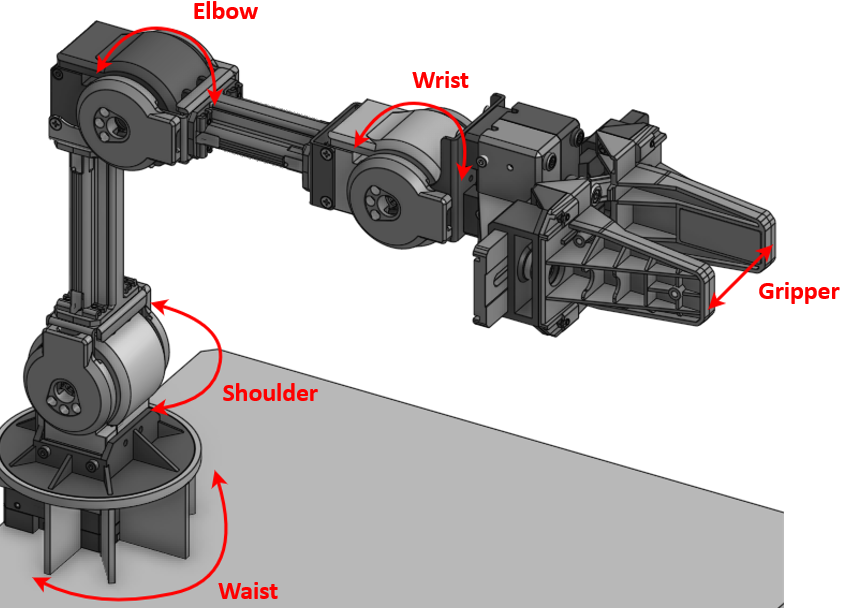
\includegraphics[width=7cm]{Arm diagram.PNG}
        \caption{Location of robotic arm joints and labels}
      \end{subfigure}%
      \begin{subfigure}{.5\textwidth}
        \centering
        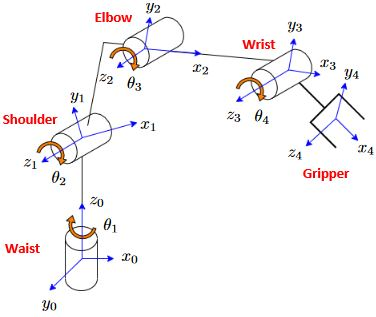
\includegraphics[width=5.9cm]{Coodinate frame.JPG}
        \caption{Initial assigment of co-ordinate frames \cite{Coordinate_frame}}
      \end{subfigure}
      \caption{}
    \end{figure}

    The actual model from which the DH table is generated is modified with the following
    design decisions:

    \begin{minipage}{.45\textwidth}
      \begin{itemize}
        \item The co-ordinate frame for the \textit{Waist} and \textit{Shoulder}
        both have the same height $z$. By setting it to the same height, it
        simplifies the final DH table since we do not have to account for the
        different heights. 
  
        \item There is a offset in the horizontal $x$ axis between the \textit{Shoulder}
        and \textit{Waist} co-ordinate frames as shown on the right. Instead of
        accounting for the $z$-axis offset and $x$-axis offset, the length of
        the hypotenus ($0.130 m$) and the angle subtended ($10.6 \deg$) is used.
        This further simplifies the resulting DH table shown in the next section.
      \end{itemize}
    \end{minipage}
    \begin{minipage}{.45\textwidth}
      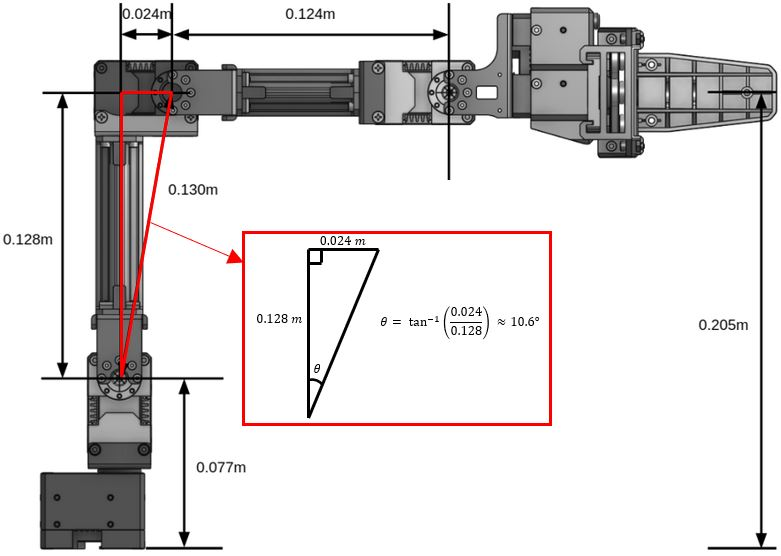
\includegraphics[width=8cm]{Offset angle.JPG}
    \end{minipage}
    
    \item The robotic arm's end effector location is designed to be in the center by default but its final position can be changed depending on the task e.g. the end effector location for drawing will be different to the end effector location for interacting with cubes.
    
\end{itemize} 

\subsection{DH Table}
The DH table is created based on the standard robotic arm position as show in Figure 1(a), and the co-ordinate frames for \textit{Waist} and \textit{Shoulder} are in the same location with different orientations.

\begin{table}[h]
    \centering
    \begin{tabular}{|c|c|c|c|c|}
    \hline
    {\textbf{}} & {\textbf{$\alpha_{i-1}$}} & { \textbf{$a_{i-1}$}} & { \textbf{$d_i$}} & { \textbf{$\theta_i$}} \\ \hline
    \textbf{Waist}           & 0                             & 0                        & 0.077                & $\theta_1$                \\ \hline
    \textbf{Shoulder}           & 90                            & 0                        & 0                    & $\theta_2 + 90 - 10.6$    \\ \hline
    \textbf{Elbow}           & 0                             & 0.130                    & 0                    & $\theta_3 - 90 + 10.6$    \\ \hline
    \textbf{Wrist}           & 0                             & 0.124                    & 0                    & $\theta_4$                \\ \hline
    \textbf{Gripper}           & 0                             & 0.126                    & 0                    & 0                         \\ \hline
    \end{tabular}
\end{table}

\subsection{Forward Kinematics}

With the DH table completed, the Forward Kinematics is implemented by
calculating the transformation matrix for each joint and multiplying them
together. This functionality is implemented as a \verb+trajectoryLib+ class
function that returns $x,y,z$ co-ordinate of the end-effector (\textit{Gripper})
when the angles for each joint is specfied. 

Referring to the \textit{Shoulder} and \textit{Elbow} in the DH table, there are
additions of $+90 \degree$ and $-90 \degree$ respectively in order to ensure the
standard pose \cite{CAD_model} is achieved with all joint angles set to $0
\degree$. This is seen in the following diagrams showing the range of rotations
for each joint with all other joints set to 0.
\begin{figure}[h]
  \centering
  \begin{subfigure}{.5\textwidth}
    \centering
    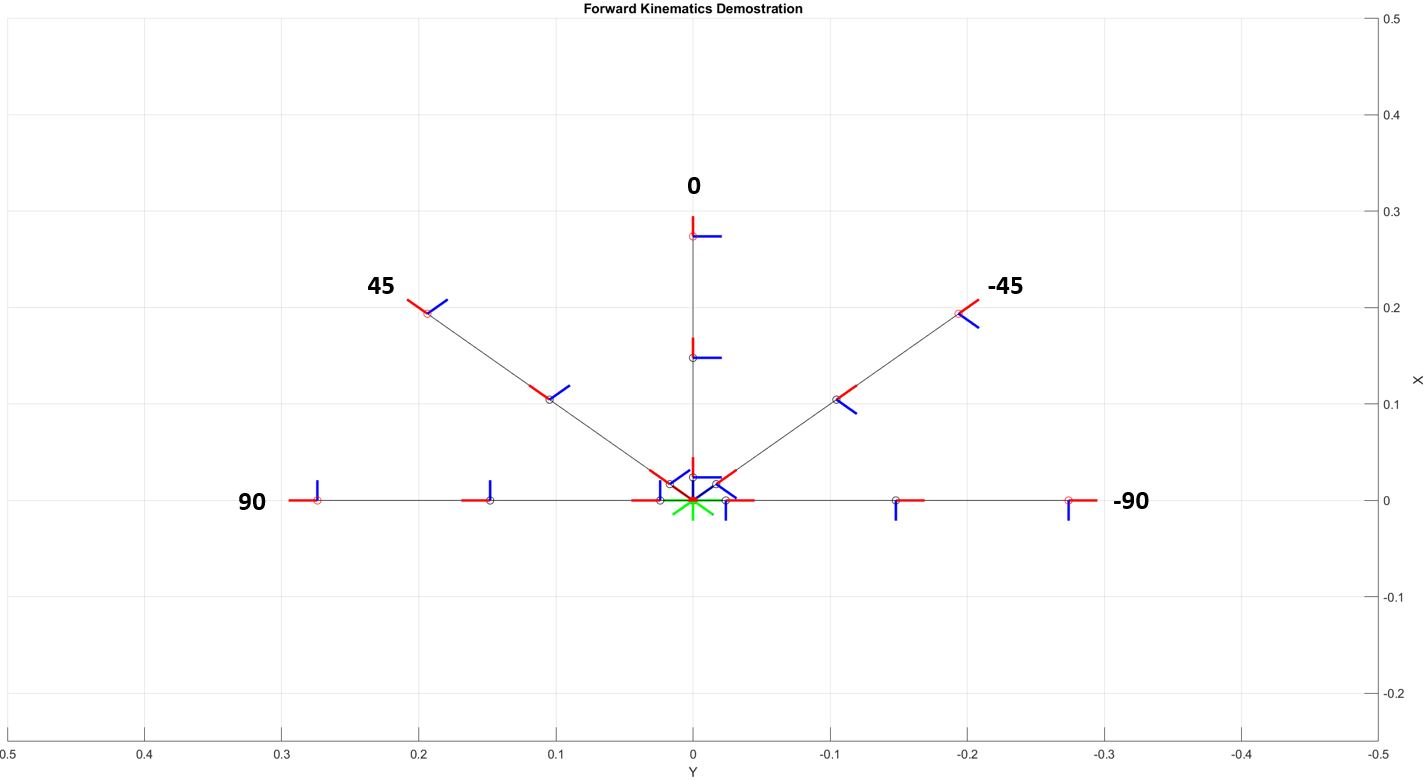
\includegraphics[width=7cm]{theta1.JPG}
    \caption{$\theta_1$ rotation: [$90\degree, 45\degree, 0\degree, -45\degree, -90\degree$]}
  \end{subfigure}%
  \begin{subfigure}{.5\textwidth}
    \centering
    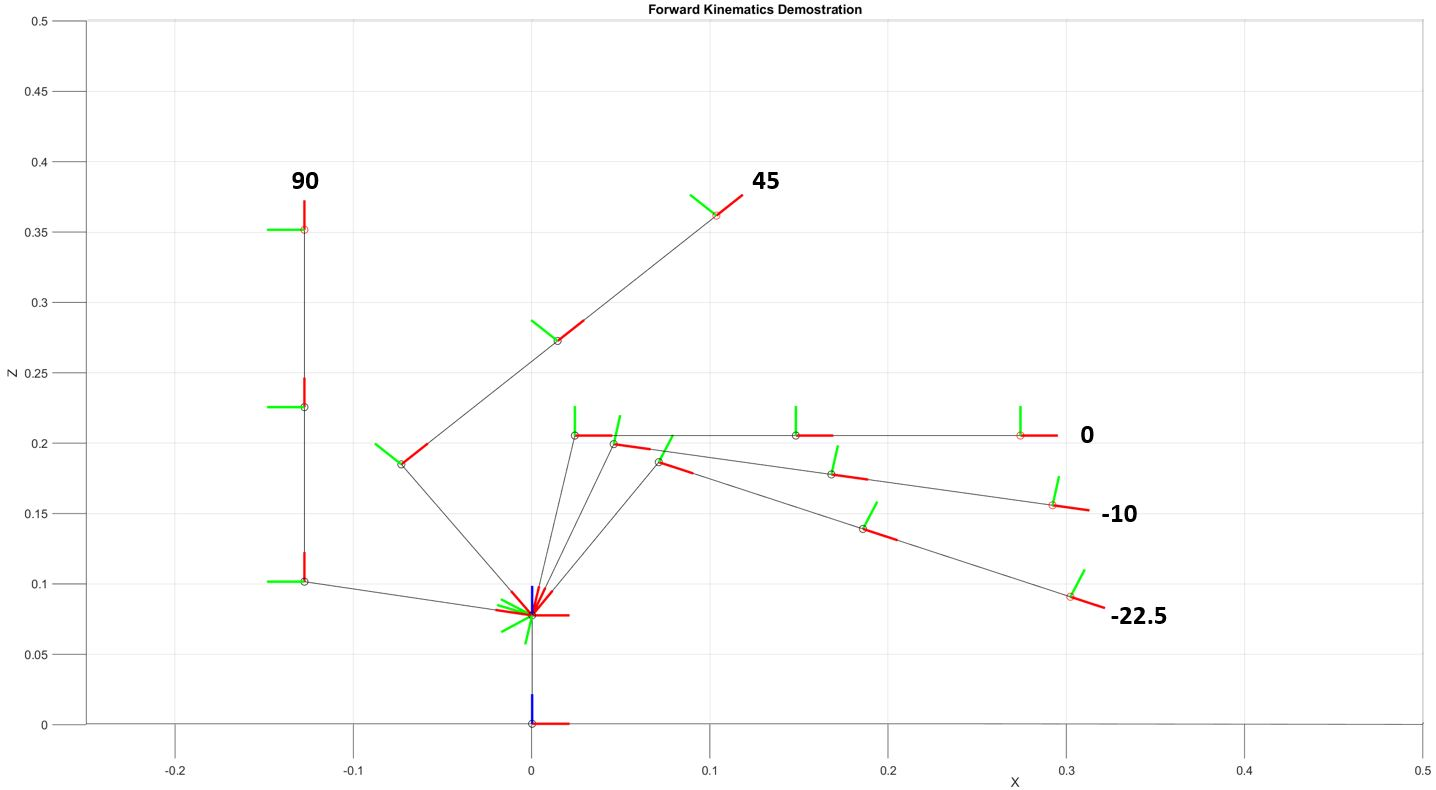
\includegraphics[width=7cm]{theta2.JPG}
    \caption{$\theta_2$ rotation: [$90\degree, 45\degree, 0\degree, -10\degree, -22.5\degree$]}
  \end{subfigure}
\end{figure}
\begin{figure}[h]
  \centering
  \begin{subfigure}{.5\textwidth}
    \centering
    \addtocounter{subfigure}{2}
    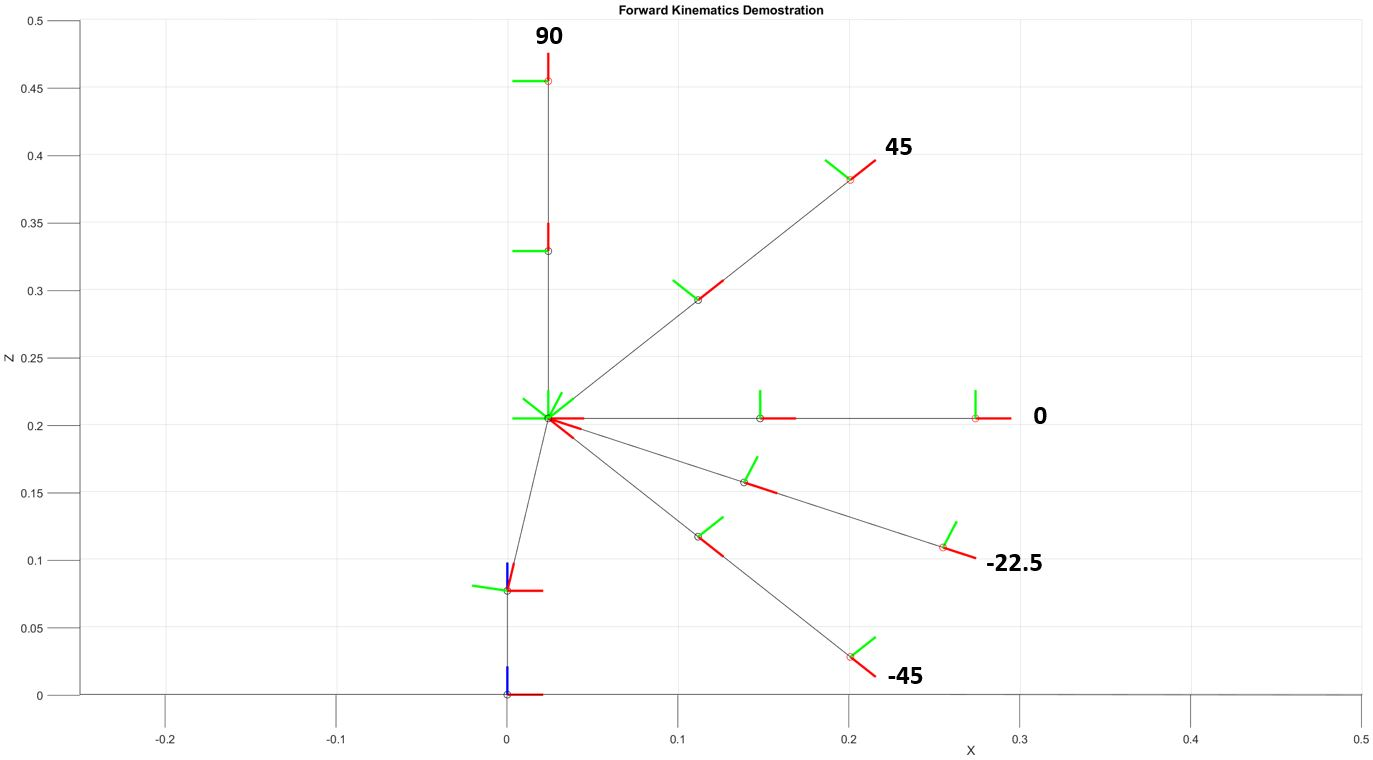
\includegraphics[width=7cm]{theta3.JPG}
    \caption{$\theta_3$ rotation: [$90\degree, 45\degree, 0\degree, -22.5\degree, -45\degree$]}
  \end{subfigure}%
  \begin{subfigure}{.5\textwidth}
    \centering
    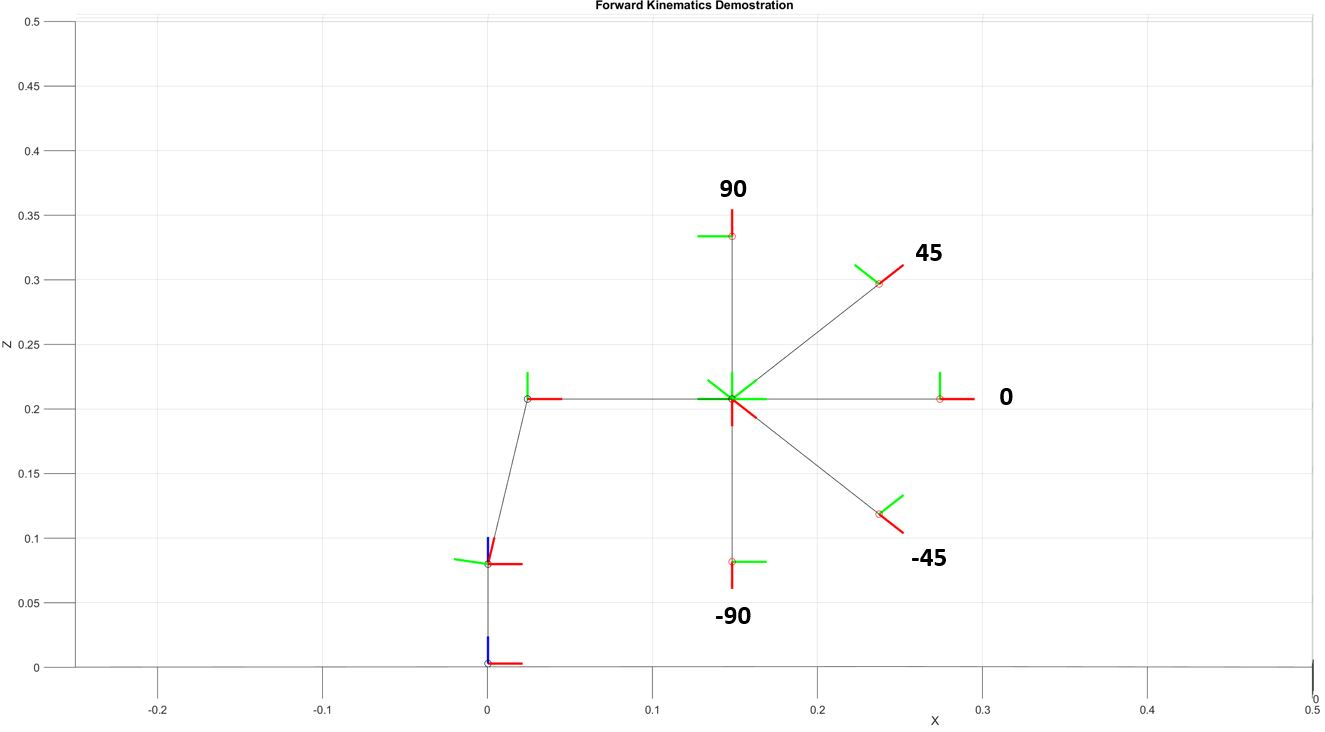
\includegraphics[width=7cm]{theta4.JPG}
    \caption{$\theta_4$ rotation: [$90\degree, 45\degree, 0\degree, -45\degree, -90\degree$]}
  \end{subfigure}
\end{figure}

\subsubsection{Implementing Joint Co-ordinate Frames}
The co-ordinate frames of the arm joints move along with the joint so the
positions of the $x,y,z$ axis is dependent on the rotation of the joints i.e. $\theta_i$
where $i$ denotes the specific arm joint. Due to this dependency, the
co-ordinate frames are implemented with a variation of Forward Kinematics where
the $x,y,z$ axis are calculated based on the $\theta_i$ value of the associated
joint. For example, the co-ordinate frame of the \textit{Waist} with rotation $\theta_1$ is calculated
using Forward Kinematics as follows:
{\small
\begin{align*}
  Waist_x &= \begin{bmatrix}
    c(\theta_1) & -s(\theta_1) & 0 & 0.021 \\ 
    s(\theta_1) & c(\theta_1)  & 0 & 0     \\ 
    0 & 0 & 1 & 0 \\ 
    0 & 0 & 0 & 1
  \end{bmatrix} 
  Waist_y &= \begin{bmatrix}
    c(\theta_1) & -s(\theta_1) & 0 & 0 \\ 
    s(\theta_1) & c(\theta_1)  & 0 & 0.021 \\ 
    0 & 0 & 1 & 0 \\ 
    0 & 0 & 0 & 1
  \end{bmatrix} 
  Waist_z &= \begin{bmatrix}
    c(\theta_1) & -s(\theta_1) & 0 & 0 \\ 
    s(\theta_1) & c(\theta_1)  & 0 & 0 \\ 
    0 & 0 & 1 & 0.021 \\ 
    0 & 0 & 0 & 1
  \end{bmatrix} 
\end{align*}
}% 
where the value $0.021$ represents the length of an axis of the co-ordinate
frame.

This functionality is implemented as a separate function
\verb+FK_coordinate_frames+ that returns the
$x,y,z$ positions relative to the joint for the 5 joints of the arm.

\pagebreak

\subsection{Inverse Kinematics}
The inverse kinematics problem for the OpenManipulator-X arm is solved through a
geometric approach that is covered in depth in the Appendix. The following
equations are the solutions to the inverse kinematics problem given co-ordinates
$(x, y, z)$:
\begin{align*}
    \textbf{Waist}: \theta_1 &= \begin{cases} 
        \arctan(\frac{y}{x}) + 180 & x < 0 \text{ and } y > 0 \\ 
        \arctan(\frac{y}{x}) - 180 & x < 0 \text{ and } y < 0 \\
        \arctan(\frac{y}{x}) & \text{otherwise}
    \end{cases} \\
    \textbf{Shoulder}: \theta_2 &= \arctan\left(\frac{\frac{L_2 + L_3*c(\theta_3)*R_2 - L_3*s(\theta_3)*R_2}{R_2^2 + Z_2^2}}{\frac{L_2 + L_3*c(\theta_3)*Z_2 - L_3*s(\theta_3)*Z_2}{R_2^2 + Z_2^2}}\right) \\ 
    \textbf{Elbow}: \theta_3 &= -\arccos\left(\frac{R_2^2 + Z_2^2 - L_2^2 + L_3^2}{2*L_2*L_3}\right)\\ 
    \textbf{Wrist}: \theta_4 &= \phi - \theta_3 - 90 + \theta_2 
\end{align*}
where: 
\begin{itemize}
    \item $\phi$ is the orientation of the end effect that is specified by the user
    \item Robotic arm lengths \cite{CAD_model}: $L_2 = 0.130$, $L_3 = 0.124$ and $L_4 = 0.126$
    \item $R_2 = |\sqrt{x^2 + y^2}| - L_4*\cos(\phi)$
    \item $Z_2 = z - 0.077$
\end{itemize}

Further conversions are required to convert the angles outputted from inverse
kinematics to the angles compatible with the openManipulator-X arm servos as
defined in the Appendix.

\subsubsection{Inverse Kinematics Simulation: Tracing a square on each cartesian plane}

To test the functionality of the inverse kinematic solver, the robotic arm draws
a cube in 3D space. The process is summarised as follows: 
\begin{itemize}
  \item Start and end co-ordinate of each line of the cube is specified 
  \item Using matlab \verb+linspace+, the co-ordinates of the points between the
  start and end points are generated 
  \item These sets of co-ordinates are concatenated together in the order the
  arm traverses over them 
  \item The combined set is iterated in a FOR loop, each co-ordinate fed into
  the \verb+IK+ function that specifies the joint angles required to acheive
  the specified co-ordinate
\end{itemize}


In the simulation, the plot also displays the joint angle values of $\theta_1$,
$\theta_2$, $\theta_3$ and $\theta_4$. 
\begin{figure}[h]
    \centering
    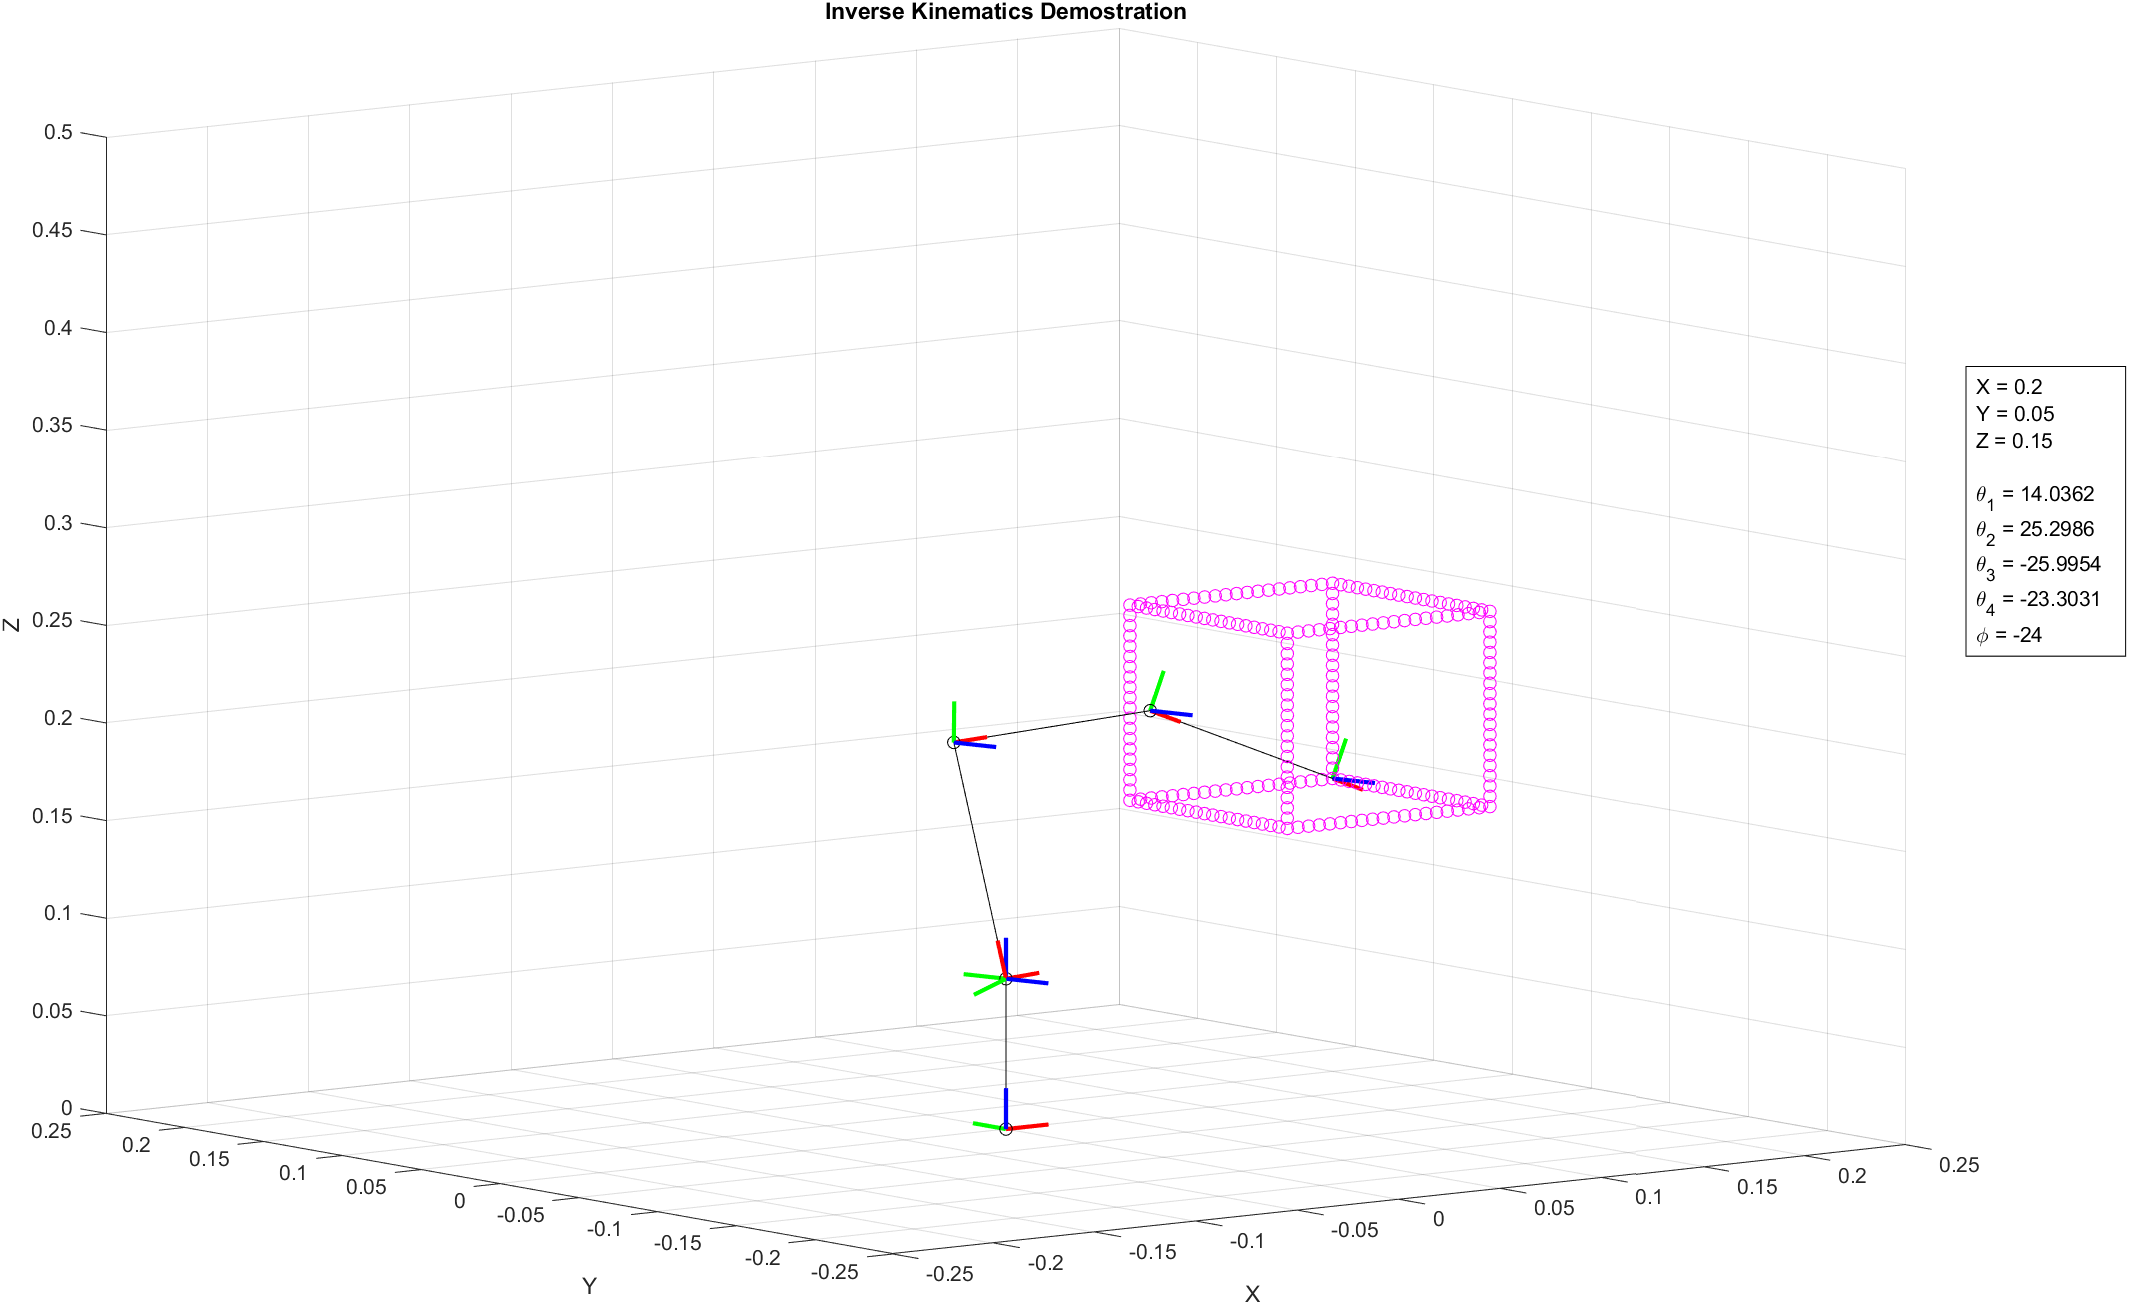
\includegraphics[width=7cm]{6}
    \hspace{1cm}
    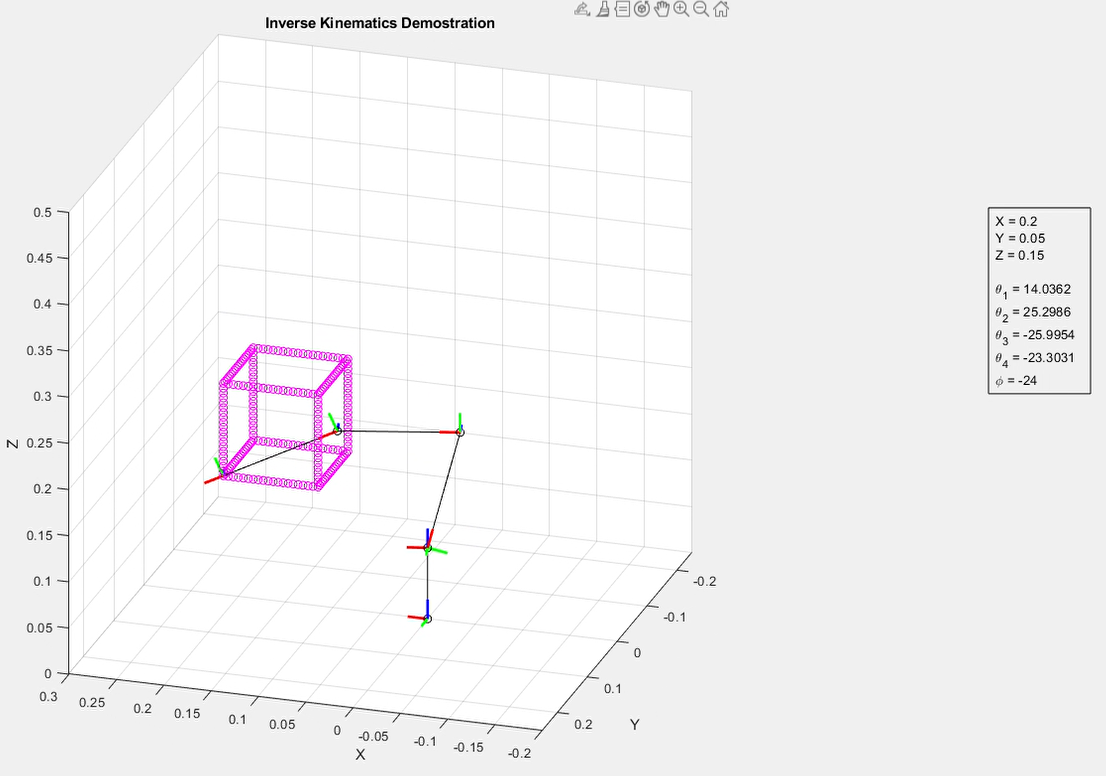
\includegraphics[width=7cm]{7}
\end{figure}

\vfill
\pagebreak

%%%%%%%%%%%%%%%%%%%%%%%%%%%%%%%%%%%%%%%%%%%%%%%%%%%%%%%%%%%%%%%%%%%%%%%%%%%%%%%%%%%%%%%%%%%%%%%%%%%%%%%%%%
\section{Task 2 - Pick and Place Cubes}

Task 2 was broken down into several modular components that enabled the team to
divide the work and tackle it separately. 
\begin{enumerate}
  \item \textbf{Picking up and dropping function}
  
  Given the $(x,y,z)$ co-ordinates of the cubes, the Inverse Kinematics solver
  will calculate the servo angles required to reach that co-ordinate. In the
  Inverse Kinematics solver, the team has added multiple checks that ensures
  only reachable co-ordinates are allowed to be fed into the arm. 
  
  For picking and dropping tasks, the team made the design decision to only pick
  up and drop cubes from the top $(\phi = -90)$. This was due to the fact that
  picking/dropping from horizontal direction $(\phi=0)$ would cause the gripper
  extrusions to hit the cube holders and increasing the height at which the
  gripper grips the cube would result in a very loose grip. 
  
  \item \textbf{Rotate cube function}
  
  Rotating cubes are divided into two types: Rotating forward and rotating
  backward. The key to completing this task was understanding that $\phi$
  determines the final orientation of the end-effector (\textit{Gripper}). With
  that, a cube can be rotated by picking it up with $\phi = 0$ and dropping it in
  the same place with $\phi = -90$, and vice versa for the opposite direction. 
\end{enumerate}
\begin{figure}[h]
  \centering
  \begin{subfigure}{.5\textwidth}
    \centering
    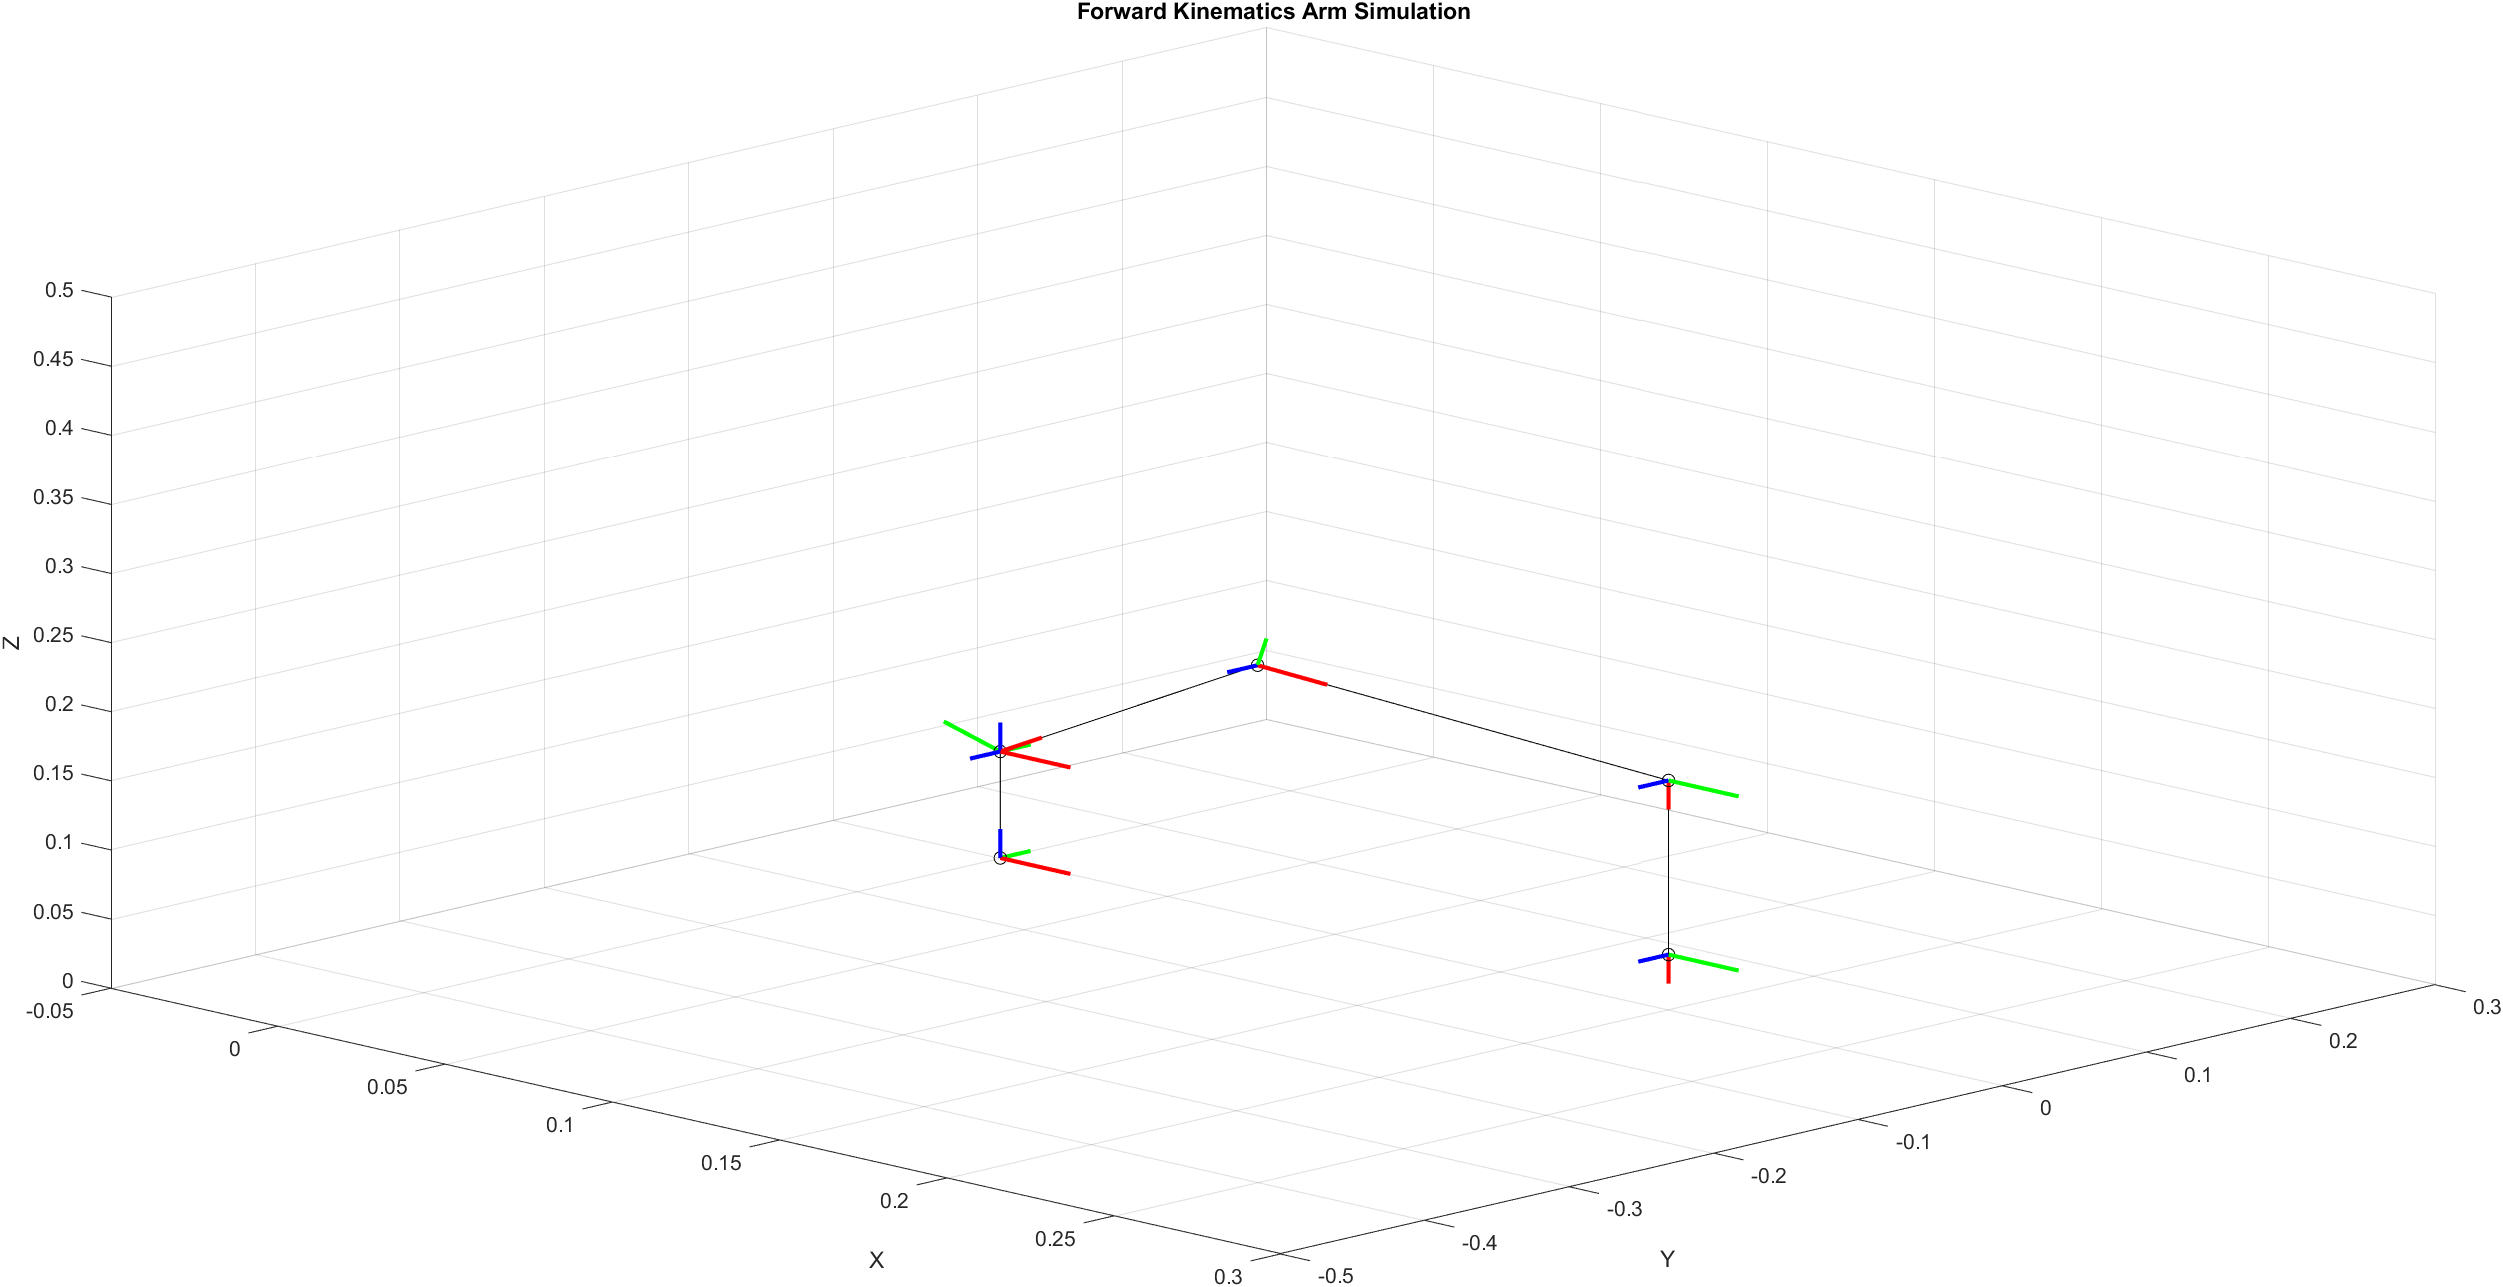
\includegraphics[width=7cm]{1}
    \caption{Picking up cube: $\phi = -90\degree$}
  \end{subfigure}%
  \begin{subfigure}{.5\textwidth}
    \centering
    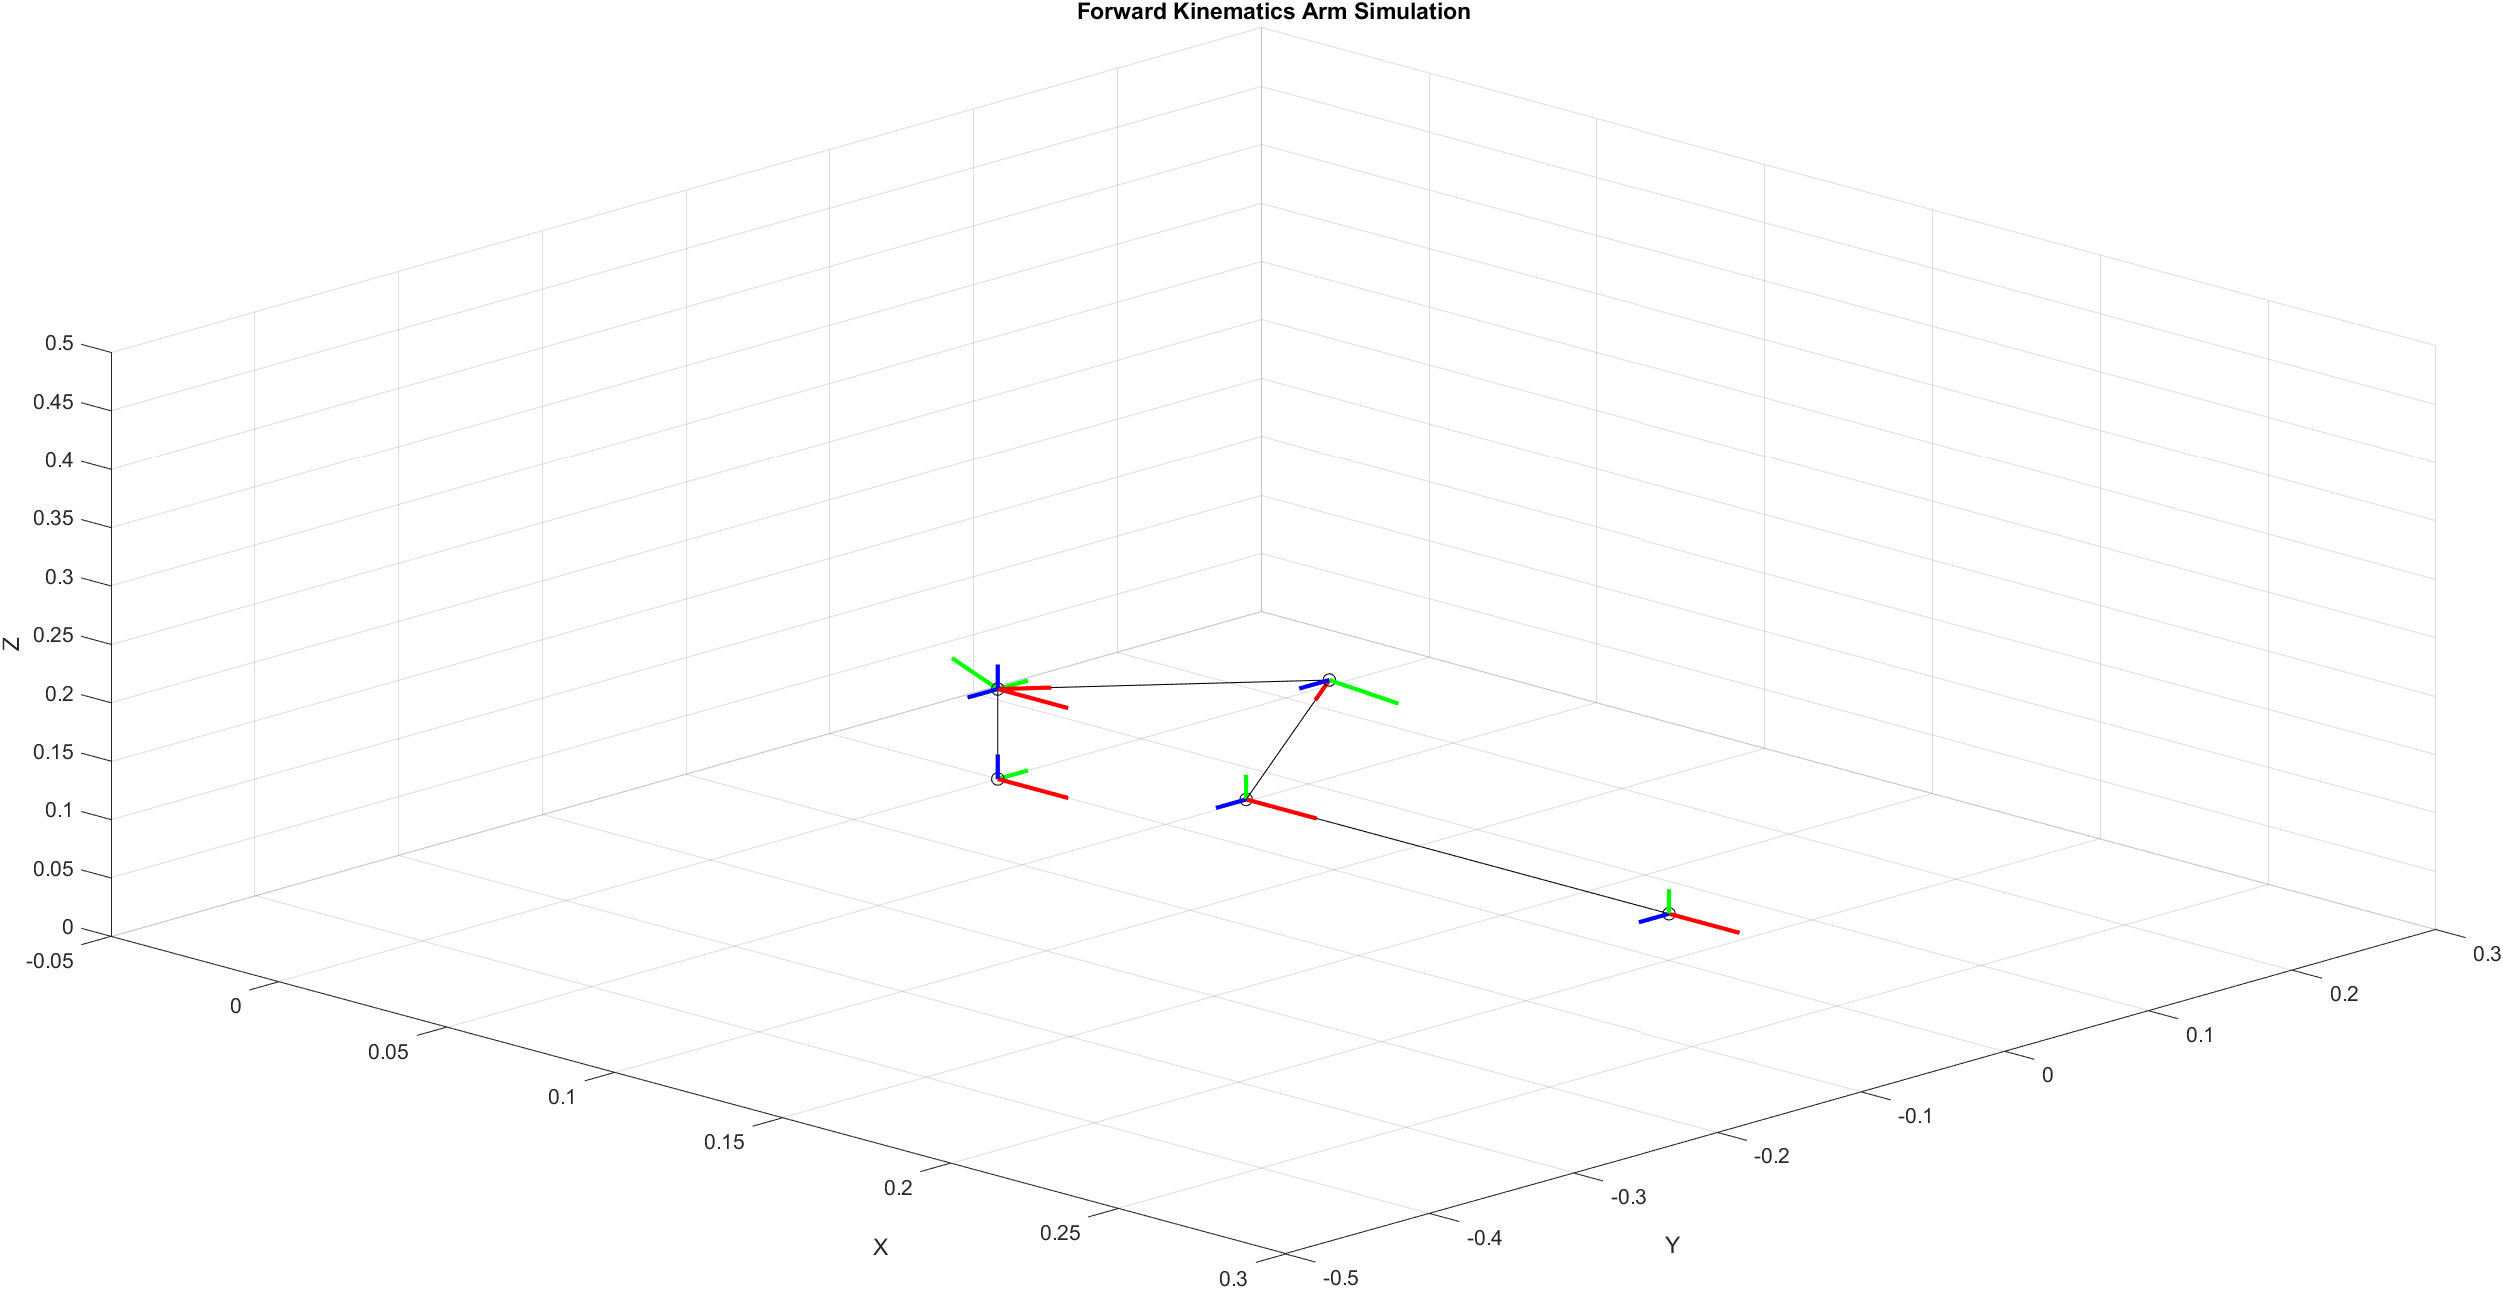
\includegraphics[width=7cm]{2}
    \caption{Dropping cube: $\phi = 0\degree$}
  \end{subfigure}
  \caption{Depiction of backward rotation}
\end{figure}

\begin{enumerate}
  \setcounter{enumi}{2}
  \item \textbf{Stacking cube function}
  
  The action of stacking is a combination of rotating and picking
  up/dropping cubes. Therefore, the arm is designed to first rotate all the cubes
  then proceed to picking up and drop the cubes at a height increasingly $0.025m$ higher to
  account for the height of the already stacked cubes. 
  
  \item \textbf{Co-ordinates of sockets on the acrylic board}
  
  With the OOP approach, the co-ordinates of every socket on the
  acrylic board could be stored as three matrices representing the $x, y$ and $z$
  values of a specific socket. To obtain the co-ordinates of a socket, the row and
  column of the desired socket is specified and the function returns the $(x,y,z)$
  co-ordinates for the associated row and column.  

  \item \textbf{Linear interpolation}
  
  Basic linear interpolation is implemented to prevent the arm moving in an
  undesired way. This is important for picking/dropping and rotating cubes where,
  without linear interpolation, could approach the cube holders from the sides
  and hit the protruded edges of the cube holders. For stacking, the behaviour
  of the arm for a particular action would be unpredictable and acidentally hit
  the stacked cubes. 

  Linear interpolation affects the action of moving down and moving up
  from cube co-ordinates. For any particular cube co-ordinate, the arm would first move to directly
  that co-ordinate with a $z$-offset of at least $+0.030m$. Once there, there
  are 3 waypoints, each with a decreasing $z$-offset where the last waypoint is
  the co-ordinate to pick up/drop off the cube. The reverse happens for the
  arm moving back up.

  For transit i.e. when the arm picks up a cube and moving to another
  co-ordinate to drop off the cube, no linear interpolation is required. The arm
  automatically determines the best way to reach the drop-off co-ordinate with a
  $z$-offset of at least $+0.030m$. 

  \item \textbf{Calibration mechanisms}
  
  
\end{enumerate}

% Talk about the calibration mechanisms present

% Talk about the linear interpolation feature 


%%%%%%%%%%%%%%%%%%%%%%%%%%%%%%%%%%%%%%%%%%%%%%%%%%%%%%%%%%%%%%%%%%%%%%%%%%%%%%%%%%%%%%%%%%%%%%%%%%%%%%%%%%
\section{Task 3 - Trajectory Following (Drawing)}

\subsection{Picking up the pen}

% CAD design 

\subsection{Drawing}

% Calculating the points - particularly focusing on the circle 

%%%%%%%%%%%%%%%%%%%%%%%%%%%%%%%%%%%%%%%%%%%%%%%%%%%%%%%%%%%%%%%%%%%%%%%%%%%%%%%%%%%%%%%%%%%%%%%%%%%%%%%%%%
\section{Task 4 - Musical instruments}

For Task 4, the team chose to perform a musical piece using drums and a
xylophone. Music is complex to the robotic arm in the sense that the timings at
which the notes are hit must be approximately correct. This meant that the
speeds of the arm servos are all different and changes continuously throughout
the musical performance. If any servos was wrongly calibrated or the arm does
not hit the instruments fast enough, the musical piece would immediately sound
wrong. This challenge was interesting to the team and we
felt that it was a suitable task to show the skills we learnt throughout the
course of this module and through working with the robotic arm. 

This task was broken down into the following steps:
\begin{enumerate}
  \item Designing the gripper to hold the xylophone stick 
  
  % CAD drawing
  
  \item Placing musical instruments in reachable range and using forward
  kinematics to note down the coordinates of drums and xylophone tone bars
  
  The DH tables are modified to account for the increased length of the end
  effector as shown below:
  \begin{table}[h]
    \centering
    \begin{tabular}{|c|c|c|c|c|}
    \hline
    {\textbf{}} & {\textbf{$\alpha_{i-1}$}} & { \textbf{$a_{i-1}$}} & { \textbf{$d_i$}} & { \textbf{$\theta_i$}} \\ \hline
    \textbf{Waist}           & 0                             & 0                        & 0.077                & $\theta_1$                \\ \hline
    \textbf{Shoulder}           & 90                            & 0                        & 0                    & $\theta_2 + 90 - 10.6$    \\ \hline
    \textbf{Elbow}           & 0                             & 0.130                    & 0                    & $\theta_3 - 90 + 10.6$    \\ \hline
    \textbf{Wrist}           & 0                             & 0.124                    & 0                    & $\theta_4$                \\ \hline
    \textbf{Gripper}           & 0                             & 0.126                    & 0                    & 0                         \\ \hline
    \end{tabular}
  \end{table}


  \item Creating functions to hit drums and specified tone bars 
  
  Functions were created that handled the actions of hitting drums and tone
  bars. With the OOP approach taken by the team, many pieces of code could be
  re-used and slightly adjusted for this particular task. This modular approach
  code allowed the team to easily identify and finely adjust factors on the fly such as
  velocity and acceleration. 
  
  \item Calibrating the hit action 
  
  \item Combining hits to produce a musical piece 
\end{enumerate}



%%%%%%%%%%%%%%%%%%%%%%%%%%%%%%%%%%%%%%%%%%%%%%%%%%%%%%%%%%%%%%%%%%%%%%%%%%%%%%%%%%%%%%%%%%%%%%%%%%%%%%%%%%
\pagebreak
\section{Appendix}
\subsection{Task 1: Inverse Kinematics}

The process to solve for the Inverse Kinematics equations is split into two
sections: $x-y$ domain and $r-z$ domain.

\subsubsection{$x-y$ domain}

The angle for the \textit{Waist} joint, given co-ordinates $(x, y, z)$ can be calculated as:
$$
  \theta_1 = \arctan \left(\frac{p_y}{p_x}\right)
$$

Note that the \textit{Waist} joint rotation range is between $-180\degree$ to
$180\degree$ with the middle point being $0\degree$. Therefore it is important
to ensure that the angles are within that range for any combination of $p_x$ and
$p_y$.
$$
\theta_1 = \begin{cases} 
  \arctan(\frac{y}{x}) + 180 & x < 0 \text{ and } y > 0 \\ 
  \arctan(\frac{y}{x}) - 180 & x < 0 \text{ and } y < 0 \\
  \arctan(\frac{y}{x}) & \text{otherwise}
\end{cases}
$$

\subsubsection{$r-z$ domain}

Angles for the \textit{Shoulder} ($\theta_2$), \textit{Elbow} ($\theta_3$) and
\textit{Wrist} ($\theta_4$) are solved in the $r-z$ domain. The $r-z$ domain is
a simplified view of the 3D space ($x,y,z$) where the $x$ and $y$ axis are
merged using the Pythagorean equation 
$$
  p_r = \sqrt{p_x^2 + p_y^2}
$$
to define the $r$ axis as shown in the image Figure 4(a).
\begin{figure}[h]
  \centering
  \begin{subfigure}{.5\textwidth}
    \centering
    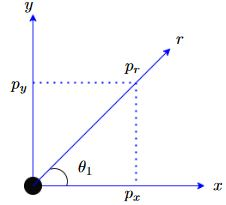
\includegraphics[width=4cm]{r.JPG}
    \caption{$r$-axis a result of merging the $x$ and $y$ axis}
  \end{subfigure}%
  \begin{subfigure}{.5\textwidth}
    \centering
    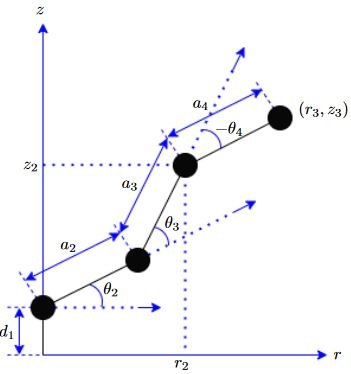
\includegraphics[width=5cm]{arm r domain.JPG}
    \caption{Robotic arm projected onto the $r-z$ domain}
  \end{subfigure}
  \caption{\cite{Coordinate_frame}}
\end{figure}

In order to solve the inverse kinematic equations, the variable term $\phi$ has
to be defined which, in this case, is defined as the sum of the angles
$$
  \phi = \theta_2 + \theta_3 + \theta_4
$$

The co-ordinates $(r_3, z_3)$ could easily be calculated given co-ordinates $(x,
y, z)$:
\begin{gather*}
  r_3 = \sqrt{x^2 + y^2} \\ 
  z_3 = z - d_1
\end{gather*}

With $(r_3, z_3)$ and $\phi$, the co-ordinates $(r_2, z_2)$ can be found:
\begin{gather*}
  r_2 = r_3 - a_4 \cos(\phi) \\ 
  z_2 = z_3 - a_4 \sin(\phi)
\end{gather*}

The \textit{Elbow} joint angle can therefore be defined as:
\begin{gather*}
  \theta_3 = \pm \arccos \left( \frac{r_2^2 + z_2^2 - (a_2^2 + a_3^2)}{2 a_2 a_3} \right)
\end{gather*}

With $\theta_3$, co-ordinates $(r_2, z_2)$ can be alternatively defined using
$\theta_2$ and $\theta_3$:
\begin{gather*}
  r_2 = a_2 \cos(\theta_2) + a_3\cos(\theta_2 + \theta_3) \\ 
  z_2 = a_2 \sin(\theta_2) + a_3\sin(\theta_2 + \theta_3)
\end{gather*}

Expanding with Ptolemy's identities:
\begin{gather*}
  r_2 = \cos(\theta_2)\left(a_2 + a_3\cos(\theta_3)\right) - a_3\sin(\theta_2)\sin(\theta_3) \\ 
  z_2 = a_3\cos(\theta_2)sin(\theta_3) + \sin(\theta_2)(a_2 + a_3\cos(\theta_3))
\end{gather*}

By recognising the hypotenus, adjacent and opposite of the triangle subtended by
$\theta_2$:
\begin{gather*}
  \cos(\theta_2) = \frac{r_2(a_2 + a_3 \cos(\theta_3)) + z_2(a_3 \sin(\theta_3))}{r_2^2 + z_2^2} \\ 
  \sin(\theta_2) = \frac{z_2(a_2 + a_3 \cos(\theta_3)) + r_2(a_3 \sin(\theta_3))}{r_2^2 + z_2^2} 
\end{gather*}

Thus the angle $\theta_2$ can be found:
\begin{gather*}
  \theta_2 = \arctan \left(\frac{\sin(\theta_2)}{\cos(\theta_2)}\right)
\end{gather*}

By using the relation of $\phi$, $\theta_2$, $\theta_3$, $\theta_4$ can be
found:
$$
  \theta_4 = \phi - \theta_2 - \theta_3
$$

\pagebreak
\section{References}
\printbibliography


\end{document}